\documentclass[twocolumn]{article}
\usepackage{usenix}
\usepackage[final]{graphicx}
\usepackage[labelfont=bf,font=footnotesize,labelsep=period,
    aboveskip=4pt plus 0.2pt,belowskip=4pt plus 0.2pt]{caption,subfig}
\usepackage{amsmath}
\usepackage[small,bottomtitles,compact]{titlesec}
\usepackage[comma,numbers,sort&compress]{natbib}
\usepackage{booktabs,tabularx,multirow}
\usepackage{algorithmic}
\usepackage{paralist}
\usepackage{ifpdf}
\usepackage[breaklinks]{hyperref}
\ifpdf
  \usepackage[protrusion=true,expansion]{microtype}
\else
  \usepackage{microtype}
\fi
\usepackage{moreverb}

\newcommand{\projectname}{Spock}
\newcommand{\linkedin}{SocialNet}

\newcommand{\doctitle}{Project \projectname{} : Batch computed read-only data serving}

\title{\doctitle}
\author{}
\date{}

\newcommand{\sql}[1]{\texttt{#1}}

\hypersetup{
    pdftitle = {\doctitle},
    pdfauthor = {},
    pdfsubject = {FAST 2012},
    pdfcreator = {LaTeX},
    bookmarksopen,
    bookmarksnumbered=true,
    pdfstartview={Fit},
    colorlinks=true,
    linkcolor=black,
    citecolor=black,
    filecolor=black,
    urlcolor=black,
}

% loosen latex's float placement parameters
\renewcommand{\topfraction}{.99}
\renewcommand{\bottomfraction}{.8}
\renewcommand{\textfraction}{.25}
\renewcommand{\floatpagefraction}{.90}
\renewcommand{\dbltopfraction}{.99}
\renewcommand{\dblfloatpagefraction}{.99}
\setcounter{topnumber}{9}
\setcounter{bottomnumber}{9}
\setcounter{totalnumber}{20}
\setcounter{dbltopnumber}{9}

% change default float positioning
\makeatletter
\def\fps@figure{t} 
\def\fps@table{t} 
\makeatother 

% make the space between the body text and a figure's caption tighter
\setlength{\textfloatsep}{4pt plus 1pt minus 3pt}
\setlength{\dbltextfloatsep}{4pt plus 1pt minus 3pt}

% make the space between adjacent floats tighter
\setlength{\floatsep}{3pt plus 1pt minus 1pt}
\setlength{\dblfloatsep}{3pt plus 1pt minus 1pt}


% subfig: tighter spacing
\DeclareCaptionOption{verytight}[]{%
    \captionsetup{farskip=0pt,topadjust=0pt,captionskip=0.2pt,%
    nearskip=0pt,margin=0pt}}
\captionsetup[subfloat]{verytight}

% paralist: fix up list spacing
\setlength{\pltopsep}{1.5pt plus 0.4pt minus 0.3pt}
\setlength{\plitemsep}{1pt plus 0.2pt minus 0.2pt}

% this will reduce the number of overfull hbox's by being more
% aggressive with paragraph formatting
\tolerance=5000
\hbadness=4000
\emergencystretch=1em
\hfuzz=.1pt
\vfuzz=\hfuzz
\widowpenalty=1000
\clubpenalty=1000

% macros that'll increase/decrease the page by a line.
\newcommand{\shortpage}{\enlargethispage{-\baselineskip}}
\newcommand{\longpage}{\enlargethispage{\baselineskip}}

% use \Nopagebreak before lists if you don't want them the previous
% paragraph to break across a page.
\makeatletter
\newcommand\Nopagebreak{\@nobreaktrue\nopagebreak}
\makeatother 

\makeatletter
\newcommand\bibsize{%
   \@setfontsize\footnotesize\@viiipt{8.75}%
   \abovedisplayskip 6\p@ \@plus2\p@ \@minus4\p@
   \abovedisplayshortskip \z@ \@plus\p@
   \belowdisplayshortskip 3\p@ \@plus\p@ \@minus2\p@
   \def\@listi{\leftmargin\leftmargini
               \topsep 3\p@ \@plus\p@ \@minus\p@
               \parsep 2\p@ \@plus\p@ \@minus\p@
               \itemsep \parsep}%
   \belowdisplayskip \abovedisplayskip
}
\makeatother

% natbib: reduce the spacing between bibliographical entries
\setlength{\bibsep}{1pt}
% natbib: reduce the references font size
%\renewcommand{\bibfont}{\bibsize}
% natbib: change punctuation of citation style
%\bibpunct{[}{]}{,}{a}{}{;}
% natbib: make the bibliography a real section, not a section*
%\renewcommand{\bibsection}{\section{\refname}}

\begin{document}

\maketitle
% ========================== ABSTRACT ==========================================
\begin{abstract}
Many internet based companies have started building analytics products backed by computationally intensive data-mining algorithms. One of the important system requirements for these products is the ability to present these results to the end user under strict latency constraints. A good systems practice to achieve this is by decoupling the computation layer from the serving layer. MapReduce paradigm, through the open-source solution Hadoop, has seen a wide spread adoption as the perfect solution for the computation layer. But it is the current serving layers which haven't been able to keep up and deal with the consumption of these massive data-sets without affecting serving performance. 

In this paper we present a fast serving and storage layer called Project \projectname{} which addresses this problem by offloading the index construction to the computation layer. We have built and open-sourced this distributed and fault-tolerant layer with the ability to serve both read-write and read-only batch computed data. In this paper we will focus primarily on the read-only data serving cycle and talk about how it has helps \linkedin{} serve multiple TBs of data regularly. With its very simple key-value based interface \projectname{} today powers most of \linkedin{}'s social recommendation products. 
\end{abstract}

\input intro.tex

% ========================== RELATED WORK ==========================================

\section{Related Work}
\label{sec:related_work}
A very common serving system used in various companies is MySQL. The two most used storage engines of MySQL - MyISAM and InnoDB - provide bulk loading capabilities into live system with `LOAD DATA INFILE' statement. MyISAM is the better amongst the two because of its compact on-disk space usage and its ability to delay the re-creation of the index to a time after the load\cite{bulk}.  Unfortunately we still have to deal with the problem of needing lots of memory, which is used for maintaining the special tree-like cache during bulk loading. 
%*\cite{http://dev.mysql.com/doc/refman/5.1/en/server-system-variables.html-sysvar_bulk_insert_buffer_size}
The other big problem with MyISAM storage engine is that it locks the complete table for the duration of the load. Hence all other requests coming in during the bulk load process are queued up. This is definitely not acceptable for web applications in general since this is equivalent to having a down-time.  

A lot of work has also been done to add bulk loading ability to some new shared-nothing cluster\cite{sharednothing} databases similar to \projectname{}. In \cite{silberstein} tackles the problem of bulk insertion into range partitioned tables in PNUTS \cite{pnuts} by adding another \emph {planning phase} to gather more statistics for the movement. Another paper from the same team \cite{pnutsbatch} shows how they used Hadoop to batch insert data faster into PNUTS.

Most of the approaches above try to optimize the bulk updates on the same indexes which are serving live traffic as well. Since we cater to static data-sets that require a complete change of the full data-set the approach we adopted was the construction of the full index offline. This alleviates the problem of us sharing any resources (like CPU and memory) with the index which is serving the live traffic. Usage of MapReduce for this offline construction has actually been a well researched idea with implementations in various production systems. The first idea of this offline construction originated in the various search systems, like Katta\cite{katta} and \cite{mika}. These search layers have hooks which trigger builds on Hadoop to generate indexes and on completion pull the indices to serve search requests. This idea has also been extended to various databases. Both \cite{konstantinou} and \cite{barbuzzi} suggested building HFiles (equivalent to SSTable files, a persistent immutable map data structure, from Google's BigTable \cite{bigtable}) offline in Hadoop and then shipping them over to be consumed immediately by HBase\cite{hbase}. This unconventional method hence bypasses the client API there-by getting rid of the problems of buffering, etc. which affects the write path. The same approach has been adopted by Cassandra\cite{cassandra} in its new \emph{sstableloader}\cite{cassandra_bulk} functionality. In general these approaches definitely alleviate the cluster from sudden memory usage pattern changes. 

But all of the above solutions don't solve one very important use case of ours. The general development pattern that we've seen for data products is that engineers come up with new algorithm tweaks and then push out the corresponding data changes in steps, while continuously monitoring their metrics. The problem kicks in when a new data load is resulting in a major drop in metrics. In such a scenario having to run a batch Hadoop job to bulk load new data back in would be very time-consuming. Our storage layout tries to solve this problem by providing some form of rollback mechanism. 
 
From an architecture perspective, \projectname{} falls into the league of many previous P2P storage systems. There have been various structured DHTs, like Chord\cite{chord} and Pastry\cite{pastry}, which provide O(log N) lookup. We are more inspired by Dynamo and Beehive\cite{beehive} which tries to decrease the variance in latency due to multi-hop routing by saving more state and providing lookups in O(1). Similar to Dynamo, \projectname{} also supports per tuple based replication for availability purposes. Updating all replicas is easy in the read-only batch scenario since these are pre-computed and then loaded into \projectname{} at once. To make replica updates fast in read-write scenario we allow our updates to some of the replicas of a key to be asynchronous. Network partitions or server failures during these asynchronous updates can result in inconsistencies between replicas. To solve this problem we version every replica and then delegate any resolution to the application during a $get$. This application level resolution has been inspired by previous work done by Bayou\cite{bayou}. 


% ========================== SYSTEM ARCHITECTURE ==========================================
\section{System Architecture}
\label{sec:system_architecture}

Before we start let us define some of the concepts and terms we will use in this paper. A \projectname{} \emph{cluster} can contain multiple \emph{nodes} (or \emph{servers}). Each server has a unique id associated with it. All the nodes in the cluster store the same number of \emph{stores} - which correspond to database tables. General usage patterns have shown that a site-facing feature may map to either one store or multiple stores. For example, a feature dealing with group recommendation may map to two stores - one storing member id to recommended group ids and second storing a group id to their corresponding description. Every store has the following list of configurable parameters:
\begin{itemize}
	\item \emph {Replication factor} - Number of servers onto which each key-value tuple is replicated
	\item \emph {Required reads} - Number of servers which we read from in parallel during a $get$ before declaring a success
	\item \emph {Required writes} - Number of server responses we block for before declaring success during a $put$
	\item \emph {Key/Value serializer and compression} - \projectname{} can have different serialization for the key and value. The various formats that we support are Avro, Protocol buffers, Thrift and Custom binary JSON. The most used format for read-only stores is our custom binary JSON format. \projectname{} also support per-tuple based compression which can be applied to key and/or value. The serialization / compression is completely dealt by a component which resides on the client side with the server only dealing with raw byte arrays. The only exception to this is a relatively new feature called `server side transforms', which will be further discussed in Section \ref{sec:system_architecture:system_components:client_api}. 
\end{itemize}


% ========================== SYSTEM ARCHITECTURE - SYSTEM COMPONENTS ==========================================

\subsection{System components}
\label{sec:system_architecture:system_components}

\begin{figure}
  \centering
    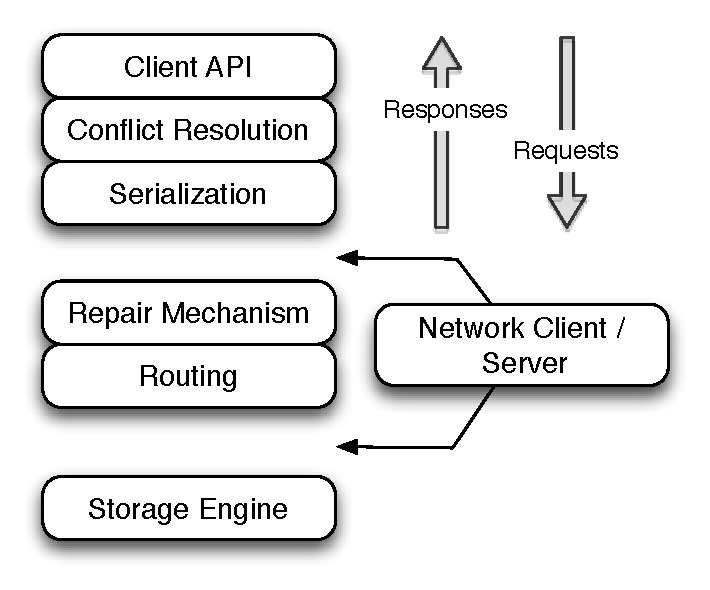
\includegraphics[scale=0.45]{images/arch.pdf}
  \caption{\projectname{} architecture stack}
  \label{arch}
\end{figure}


Since \projectname{} has been inspired from Amazon's Dynamo paper, we have a similar pluggable architecture. Figure \ref{arch} shows the high level architecture of \projectname{}. Each box represents a module, all of which share the same simple code interface. Every module has exactly one functionality, which we'll explain in the following sub-sections. This type of layering makes it easy to interchange modules and place them in any order. For example we can have the routing module on either the client side or the server side. Functionality separation at module level also allows us to easily mock these modules for testing purposes. One of the most common use of this can be found in our unit tests where we mock the storage layer to use an in-memory hash map based engine for quick results.  

% ========================== SYSTEM ARCHITECTURE - SYSTEM COMPONENTS - CLIENT API ==========================================

\subsubsection {Client API }  
\label{sec:system_architecture:system_components:client_api}

Starting from the top our client has a simple $get$ and $put$ API with no support for complex operations like joins, foreign key constraints, etc. Here are the functions that we provide. 

\scriptsize
\begin{verbatim}
VectorClock<V> get (K key)
put (K key, VectorClock<V> value)
VectorClock<V> get (K key, T transform)
put (K key, VectorClock<V> value, T transform)
\end{verbatim}
\normalsize

The first two functions are simple except we version every tuple with a vector clock (more about this in Section \ref{sec:system_architecture:system_components:conflict_resolution}). The next two functions show a very powerful feature in \projectname{} which allows you to run a transform / function on your data when it is on the server side. Correctly using this can help us in saving some network bandwidth by transferring only the required parts of a large value. A common example of this is when we have a list of entities as the value. We can then run a transformed $get$ to only retrieve a sub-list or a transformed $put$ to append an entity to your list. 

% ========================== SYSTEM ARCHITECTURE - SYSTEM COMPONENTS - ROUTING LAYER ==========================================

\subsubsection {Routing layer }  
\label{sec:system_architecture:system_components:routing_layer}

Before we talk about conflict resolution it is important we understand how routing and replica assignment works. Since \projectname{} can be thought of as a massive hash table we need a way to partition the data across the multiple servers. The best partitioning implementation would be one which would split the `hot' set of data into minute chunks and spread them across such that they fit in memory on the individual servers. Also server failures, maintenance or just being overloaded are common scenarios. In such cases we definitely don't want our clients to stop serving data. This motivates the need to also replicate the data onto multiple servers. 

The Dynamo paper solved both these problem by using `virtual nodes' along with consistent hashing. The initial approach they took was to visualize the integer hash values as a ring beginning at 0 and circling around to some max value (if we use MD5 as our hash, 128 bits = 2$^{128}$-1). Then each node is assigned an integer which is in turn hashed into this ring multiple times (each location of it is called a token). Then each node becomes responsible for the region between its token and the predecessor token (belonging to another node) on the ring. A key is assigned to a node by hashing the key to yield its position in the ring and then jumping the ring clockwise to find the first token (and hence node) with a greater hash value. Similarly the replicas are decided by jumping further till you find `replication factor' (\verb=N=) number of tokens belonging to different nodes. This list of nodes is called the `preference list' for the key. This consistent hashing approach has the advantage that if a node goes down the affected keys are only ones hashed to regions close to the tokens belonging to the dead node. The disadvantage is that we may result in unequal key ranges because of the uneven hashing of the tokens thereby resulting in a skew. 

To solve this problem the better approach is to instead split the hash ring into equal size `partitions' and then assign these partitions to nodes. We share this ring with all the stores, which means changes in the ring require us to change all the stores. Now to generate the preference list we first hash the key to a range belonging to a partition and then continue jumping the ring clockwise till we find \verb=N=-1 other partitions belonging to different nodes. This equal sized range based approach helps solve the imbalance key range problem. It also indirectly helps in data-management (as further discussed in Section \ref{sec:read_only:data_cycle:rebalancing}) since having segregated logical file groups for a partition can help with rebalancing. 

Since our routing layer is customizable it was easy to plug in another variant of the above consistent hashing algorithm to support routing in multiple data-center environment. For the same we start by grouping nodes into logical clusters that we call `zones'. A zone in the real world can be a data-center, a rack or just a group of nodes close together. Besides this we have a `zone proximity list' which contains information regarding zone distances (For example, Zone A is closer to Zone B than Zone C). Now we provide the user the ability to decide how many replicas they want per zone and then while generating the preference list jump the ring to find partitions belonging to different nodes and zones. Once the routing module generates the preference list it reorders it depending on the proximity list of the zone it is present in. This enables us to make sure requests first go to local zones instead of remote zones. 

Figure \ref{hash} is an example of how the two routing strategies would generate different preference lists for the same key.  

\begin{figure}
  \centering
    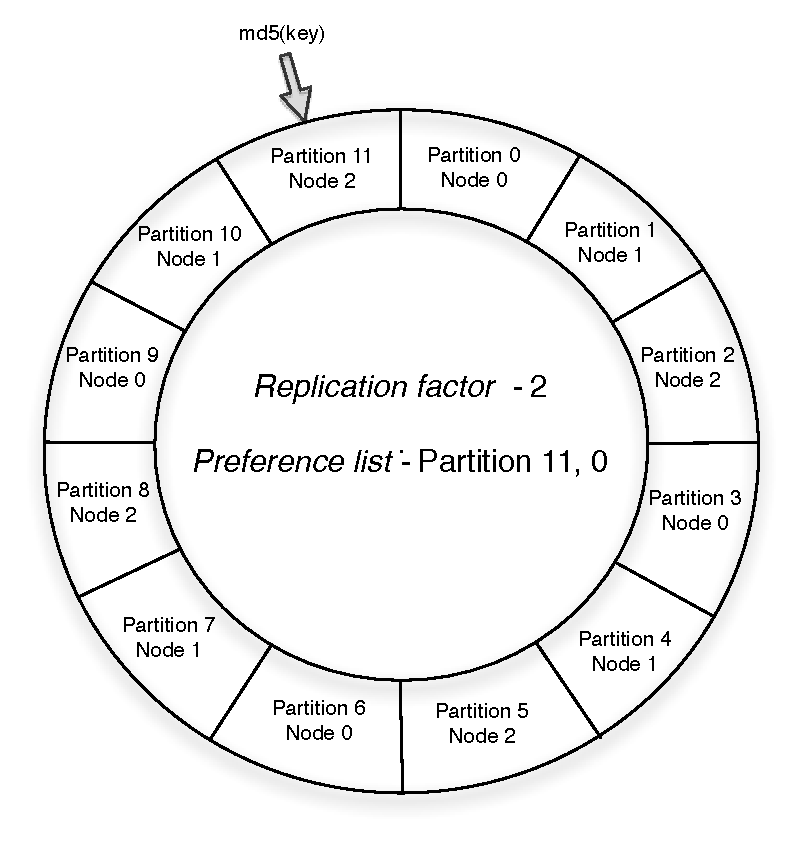
\includegraphics[scale=0.55]{images/hash.pdf}
  \caption{Hash Ring}
  \label{hash}
\end{figure}

% ========================== SYSTEM ARCHITECTURE - SYSTEM COMPONENTS - CONFLICT RESOLUTION ==========================================

\subsubsection {Conflict Resolution } 
\label{sec:system_architecture:system_components:conflict_resolution}

In distributed systems network partitions are possible. In such scenarios if you are updating various replicas of the same key it becomes very essential that we have some form of versioning in order to resolve future conflicts. In particular these versions should be able to differentiate between overwrites and conflicts. 

For the same we use the concept of vector clocks \cite{lamport}. A vector clock keeps a counter for each writing server, and allows us to calculate when two versions are in conflict and when one version succeeds or precedes another. In practice this is a list of node id and counter pair. These counters are incremented depending on which node acts as the pseudo-master for a request. For example,  $[1:10,2:3]$ signifies that node id 1 was master for this replica 10 times while node id 2 was 3 times. 

The use of vector clocks also allows us to support some form of optimistic locking on the client side. For example, if two clients both try to update the same key with the same vector clock only one of them will succeed while the other will be thrown a special error. This special error can then trigger the client to do the same $get$ and $put$ operation again some number of times, but now with the updated vector clock. We call this $applyUpdate$ and have seen its usage in various applications that require a `read, modify, write if no change' loop (Eg. counters)

% ========================== SYSTEM ARCHITECTURE - SYSTEM COMPONENTS - CONSISTENCY MECHANISM  ==========================================

\subsubsection {Consistency Mechanism }
\label{sec:system_architecture:system_components:consistency_mechanism}

When doing multiple simultaneous writes distributed across multiple servers consistency of data becomes a difficult problem. The traditional solution to this problem is distributed transactions, but these tend to have two problems. Firstly they are very slow due to the multiple round trips required for handshakes and acknowledgements. The other problem with them is that they tend to be very fragile and cannot work if some of the servers are down. One solution to this problem is to tolerate the possibility of inconsistency and provide mechanisms of eventually catching up on all the missed updates. 

For the same we provide two consistency mechanisms in \projectname{} for read-write stores - read repair and hinted handoff. Read repair method detects these inconsistencies during read-time (using vector clocks) and resolves the problem by doing asynchronous writes. The other consistency mechanism, hinted handoff, is triggered during write time. If during a $put$ we find that some of the destination nodes are down (and we have satisfied our `required writes') the client triggers an asynchronous write to a special store called `slop store' on one of the live nodes. We write a `hint' to this store - where a hint contains the node id of the down node along with the updated value that it missed. We then have a periodic background job running on every node which tries to push these `hints' out to the down nodes.

% ========================== SYSTEM ARCHITECTURE - SYSTEM COMPONENTS - STORAGE ENGINE  ==========================================

\subsubsection {Storage engines}
\label{sec:system_architecture:system_components:storage_engine}

The storage layer is pluggable with a simple interface which all storage engines must implement. Besides the basic $get$ and $put$ functions every storage engine must also implement the following two functions 

\scriptsize
\begin{verbatim}
Iterator<K> keys() 
Iterator<Pair<K, VectorClock<V>>> entries()
\end{verbatim}  
\normalsize

This allows us to provide streaming get API which can be helpful for debugging as well as rebalancing. The various storage engines that \projectname{} supports are Berkeley DB Java Edition, in-memory hash map, MySQL, Krati and our custom read-only storage engine. 

% ========================== SYSTEM ARCHITECTURE - SYSTEM COMPONENTS - ADMIN SERVICE  ==========================================

\subsubsection{Administrative service}
\label{sec:system_architecture:system_components:admin_service}

Besides running the above stack every node also runs a special service on every node which allow administrators to run special commands. Here we list some of the commands that we support.

\begin{itemize}
	
	\item \emph{Add / delete / truncate store} - Ability to add or delete a store without down time. We can also truncate the complete data without deleting the store. 
	\item \emph{Stream data} - We have the ability to stream data out of a store. If the store is read-write, we can stream data in as well. 
	\item \emph{Read-only store operations} - Trigger the batch fetch from Hadoop as well as other related operations. We will discuss this further in Section \ref{sec:read_only}. 
	\item \emph{Slop operations} - Ability to manually trigger the periodic pushing job for hinted handoff. 
	
\end{itemize}

\begin{figure}
  \centering
    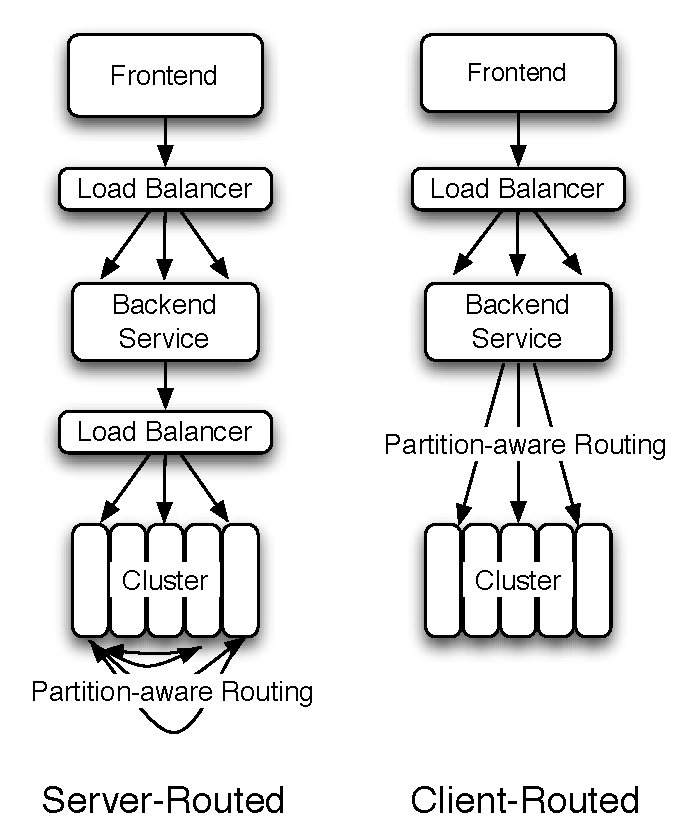
\includegraphics[scale=0.60]{images/fullstack.pdf}
  \caption{\projectname{} in full stack}
  \label{fullstack}
\end{figure}


\noindent 
Now that we know the individual components, let us look at how \projectname{} is being used inside the complete \linkedin{} stack. As shown in Figure \ref{fullstack} we support both server side as well as client side routing. Client side routing requires an initial `bootstrap' step where-in it needs to retrieve two pieces of metadata - the cluster topology metadata and the store definitions. Since both of these are persisted on each and every \projectname{} node, the client initially hits a load balancer which in turn picks up a random live node to bootstrap from. Once the metadata has been retrieved the client gets the benefit of doing one less hop compared to server side routing since it knows exactly where the replicas for a key are. This is beneficial from a latency as well as throughput perspective since we have less number of services acting as bottlenecks. The disadvantage of the client side routing is that it makes the client side code-base large because of the extra routing and replication logic. Also, as we'll further explain in Section \ref{sec:read_only:data_cycle:rebalancing}, it also makes rebalancing of data complicated since we now need a mechanism to change the cluster topology metadata on these live clients. 

% ========================== READ-ONLY-STORAGE ENGINE  ==========================================

\section{Read-only storage engine}
\label{sec:read_only}

Before we started writing our own custom storage engine we decided to
evaluate currently available storage engines, MySQL and Berkeley BD
(BDB), to see if they could fit our bulk loading use-case. Our
criteria for success was the ability to bulk load data as fast as
possible with minimum disk space overhead while still serving live
traffic.
 
We started by evaluating the various storage engines provided by
MySQL. The na\"ive approach of multiple insert statements is
problematic as every statement results in an incremental change to the
underlying index structure---in this case, a B$^{+}$ tree---which in
turn results in many disk seeks. To solve this problem, MySQL provides
a \sql{LOAD DATA} statement that tries to bulk update the underlying
index, but this requires a lock of the entire table if we the MyISAM
storage engine is used. InnoDB supports row-level locking, but comes
at the expense of substantial disk space overhead for every tuple.
Further, to achieve MyISAM-like performance with InnoDB, data must be
ordered by primary key.

We tried completely offloading the index construction to another
system as building the index on the serving system has isolation
problems, particularly with CPU and I/O. We attempted to build MyISAM
stores offline, opting to skip InnoDB due to the huge space
requirements. To do so, we leveraged the fact that MySQL allows
copying of database files from another node into a live database
directory; thereby automatically making it available for serving. We a
separate cluster where-in we would bulk load and then eventually copy
the data over to the live cluster, but this requires an extra
maintenance cost of a separate MySQL cluster with exactly the same
number of nodes as the live one. Further, the lack of ability to load
compressed data directly makes this process more time consuming, as
the data is copied multiple times between nodes: once as a flat file
to the bulk load cluster, then the internal copy during the LOAD
statement, and finally the raw data copy to the actual live database. 

The previous solution is not ideal due to its dependency on the
redundant MySQL servers, which makes the complete process prone to
failure downtimes. Instead, what if we could use the inherent fault
tolerance and parallelism of Hadoop and build individual node /
partition level data stores which could be pulled over by
\projectname{} for serving? The large-scale adoption of HDFS as the
data sink makes it an ideal location to act as our source of data:
most data is ETL'd into HDFS for storage and later processing anyway.
So the next attempted approach was to use Hadoop and a good single
node node high performance storage engine to generate smaller data
stores in parallel. That is, a Hadoop job reads data from a source in
HDFS, re-partitions on a per node basis, and finally writes the data
to individual stores (for example, BDB) on the local filesystem in the
reducer phase. The number of reducers were equal to the number of
nodes, but could have easily been further split on a per partition
basis. This data is then read from the local filesystem and copied
onto HDFS from where it can be read by \projectname{}. The benefits of
this approach is that it leverages Hadoop's fault tolerance to build
the indexes offline, but it suffers from an extra copy from the local
file system the reducer nodes to HDFS---which can become a real
bottleneck with terabytes of data. 

From the above experiments we came to the conclusion that we required
our own custom storage engine. Our new custom storage engine, along
with its complete pipeline, should have the following properties. 
\begin{compactitem}
\item \emph{No performance impact on live requests}. The incoming
requests to the live store must not be impacted during the data load.
There is a tradeoff between modifying the current index on the live
server and finishing the bulk load as fast as possible, but that can
increase I/O and hurt performance. As a result, we completely rebuild
the index offline. 
\item \emph{Fault tolerance and scalability}. Every step of the data
load pipeline should be able to handle failures. Hadoop, but its
ability to deal with failures, is used as the computation layer for
building the index. Similarly, HDFS's replication provides
availability. Finally \projectname{} is used as the serving layer, as
its routing strategies provide replica fall back in the case of
failures. All of these systems can easily scale horizontally due to
their already existing support for expansion without downtime. 
\item \emph{Rollback}. The general trend we notice in our business
that data is treated more like code: incorrect or incomplete data
could have been due to algorithm changes or source data problems. To
minimize the time in error, the storage engine must support very fast
rollback to the previous dataset.
\end{compactitem}

Our new data deployment pipeline consists of a new storage engine that
is built in Hadoop (\S\ref{sec:read_only:storage_format}), versioned
for rollback (\S\ref{sec:read_only:versioning}), and deployed. We
finally conclude by explaining how it fits into the complete data
deployment cycle along with some real world production scenarios and
how we dealt with it. 

% ========================== READ-ONLY-STORAGE ENGINE  - STORAGE FORMAT ==========================================

\subsection{Storage format}
\label{sec:read_only:storage_format}

A quick study of previous literature showed that most storage formats try to build data structures that keep the data memory-resident in the process address space. Unfortunately most of them do not think too much about caching being done by the operating system's page cache. Classical example of this is InnoDB storage engine of MySQL which buffers both key and data pages resulting in double caching 
% \cite{Page 203 - Understanding MySQL internals} 
at both OS as well as MySQL level. Also the latency gap between access from page cache vs disk is so massive that the only real performance benefit by maintaining our own structure would be for elements already in the page cache. In fact now this custom structure may even start taking memory away from the page cache. This motivated us to build our storage engine to exploit the page cache instead of maintaining our own complex data structure. Since our data is immutable the simplest way to do so is by memory mapping the entire index into the address space. Since \projectname{} has been written in Java and runs on the JVM, delegating the memory management to the operating system is also a big plus point since we now don't need to worry about Java's garbage collection and its tuning.

The following diagram is the structure of our storage engine's data and index files. 

\begin{figure}
  \centering
    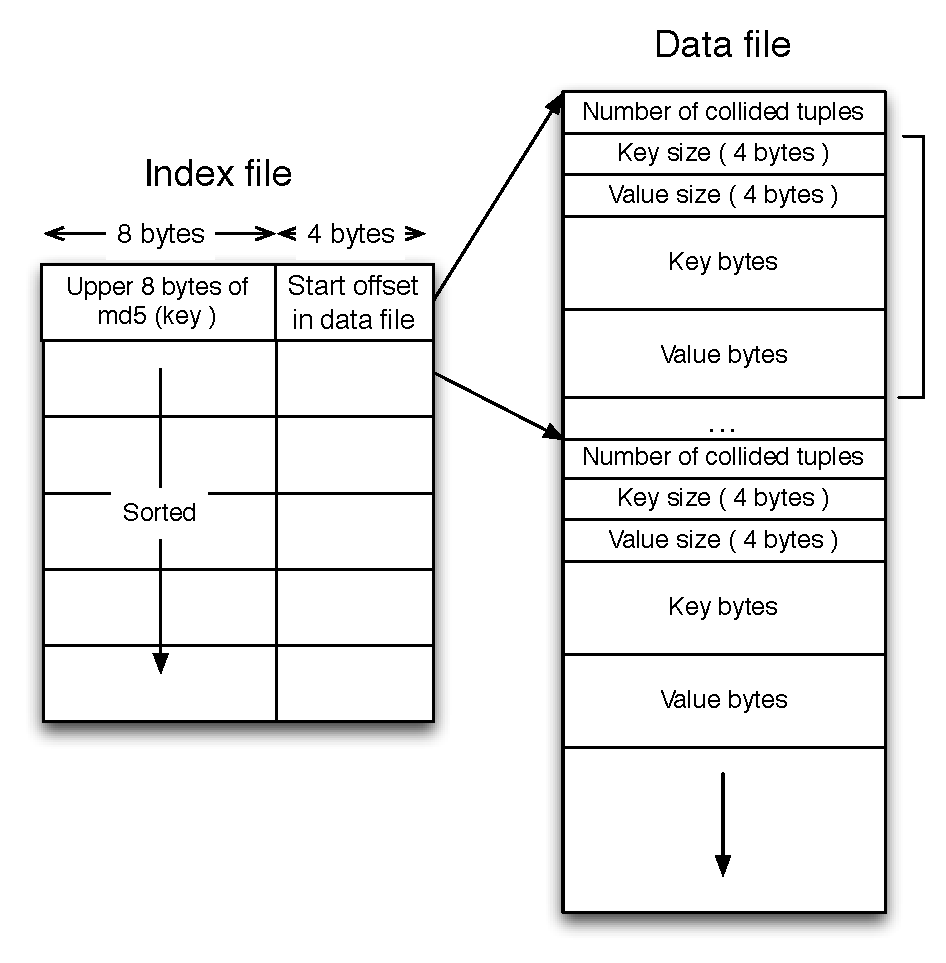
\includegraphics[scale=0.45]{images/storage_format.pdf}
  \caption{Chunk file format}
  \label{storage_format}
\end{figure}


We split our data into multiple chunks where every chunk is a pair of data and index file. There are two reasons to split the data into multiple chunks - (a) parallelism achieved on the Hadoop side (b) limitation of Java to memory map files up to a maximum of 2 GB. We build multiple chunks for every partition-replica bucket. We have set a standard naming convention for all our chunk files. It follows the pattern \verb=<partition id>_<replica id>_<chunk id>.= \verb=<data or index>=, where \verb=partition id= is the id of the primary partition and \verb=replica id= is a number between 0 to `replication factor'-1. Once a key hashes to a particular node, we classify it into the correct \verb=partition id= + \verb=replica id= bucket. For example the key in Figure \ref{hash}, present in a store using consistent hashing, would fall into the buckets 11\_0 (on node 2) and 11\_1 (on node 0). 

We then take all the tuples in this bucket and split it up into multiple smaller chunks. The table \ref{tab:node_to_chunk} below shows the various bucket names (where every bucket will contain multiple chunks and each chunk will in turn contain an index and data file) for a store with consistent hash routing and replication factor 2. This assumes that the cluster has the same partition ring topology as shown in Figure \ref{hash}. This bucket granularity was definitely not present in our first iteration since we had initially started by defining a bucket to be only on a per node basis (i.e. multiple chunks stored on a node with no knowledge about partitions). Over time we realized that breaking up the bucket into smaller granularity would help rebalancing. We will describe this in more details in Section \ref{sec:read_only:data_cycle:rebalancing}. 

\begin{table}
\begin{center}
    \begin{tabular}{ | c | c | }
    \hline
    Node Id & Chunk files \\ \hline
    0 &  0\_0, 3\_0, 6\_0, 9\_0,      2\_1, 5\_1, 8\_1, 11\_1	\\
   1 &   1\_0, 4\_0, 7\_0, 10\_0,      0\_1, 3\_1, 6\_1, 9\_1		\\
   2 &    2\_0, 5\_0, 8\_0, 11\_0,    1\_1, 4\_1, 7\_1, 10\_1		\\
\hline
    \end{tabular}
\end{center}
 	\caption{Node to chunk mapping}
 	\label{tab:node_to_chunk}
\end{table}


The index file is a compact structure containing sorted upper 8 bytes of the MD5 of the key followed by the 4 byte offset of the corresponding value in the data file. The primary reason to go for this simple sorted structure, in comparison to various previous complicated page aware structures described in literature, was to keep the build process simple. Since we wanted to leverage Hadoop for our index construction we had to face the inherent limitation that generally mapper and reducer tasks do not have much memory. Building complicated structures then would require us to explore various fancy external tree building functions thereby making the process very error prone. Preliminary tests also showed that the index files were generally order of magnitude smaller than the data files. Hence we could safely assume that they would fit into page cache easily. 

We had initially started by using all 16 bytes of the MD5 of the key in the index file. But over time as we started on-boarding various new stores we started getting performance problem. This was happening because having lots of stores was resulting in stamping on each others pages in the page cache. To alleviate this problem we needed to cut down on the amount of data being memory mapped. This could be achieved by cutting down on the number of bytes of the MD5 of the key and accepting collisions in the data file. So we wanted to find the right number of bits which would result in minimum number of collisions. This problem could easily be mapped to the classic birthday paradox problem,  which says that if we want to retrieve \verb=n= random integers from a uniform distribution of range \verb=[1, x]=, the probability that at least 2 numbers are the same is  $(1 - e^{\frac{-n(n-1)}{2x}})$. Mapping this to our read-only stores scenario, our \verb=n= is generally our 120 million member user base, while the initial value of \verb=x= was equal to $2^{128} - 1$ (16 bytes of MD5 = 128 bits). The probability of collision in this scenario was close to 0. Now if we try to decrease this to say 4 bytes (i.e. 32 bits), this gives a very high collision probability of $(1 - e^{\frac{(-120*10^{6} * (120*10^{6} - 1)}{2 * (2^{32} - 1)}}) \sim 1$. But if we instead cut it by half to 8 bytes (i.e. 64 bits) we get a very low probability of $(1 - e^{\frac{(-120*10^{6} * (120*10^{6} - 1)} { 2 * (2^{64} - 1 )}}) \sim 3.9024e^{-04}$. The probability of more than one collision is even smaller. In conclusion, by decreasing the number of bytes of the MD5 of the key we were able to cut down the index size by 40\%, thereby making our clusters more multi-tenant. Unfortunately this came at the expense of us having to (a) save the keys in the data file to use for lookups (b) take care of rare collisions in the data files.

The data file is similarly a very highly packed structure where we store the number of collided tuples followed by a set of collided \verb=[key size, value size, key, value]= list. The important thing to remember here is that we store the raw key bytes instead of the MD5-ed key bytes in order to do a comparison during reads. 


% ========================== READ-ONLY-STORAGE ENGINE  - VERSIONING ==========================================

\subsection{Versioning of data}
\label{sec:read_only:versioning}

One of our requirements was the ability to rollback the data. The above chunk files need to be stored in a layered format so as to allow us to do rollback. Every time the user creates a new copy of the complete data-set we need to demote the previous copy to an older state but still keep it around in case of a scenario of rollback. Following is how the data is structured for the read-only stores on a \projectname{} node. 

\scriptsize
\begin{verbatimtab}
store_name/
  version-2/
    .metadata
    0_0_0.data
    0_0_0.index
    ...
    100_0_0.data
    100_0_0.index
  version-3/
    .metadata
    0_0_0.data
    0_0_0.index
    ...
    100_0_0.data
    100_0_0.index
  latest -> version-3
\end{verbatimtab}
\normalsize

Every store is represented by a directory which then contains various `versions' of the data. Since the data in all the version directories, except the serving one, are inactive we are not affecting the page cache usage and hence the latency. Since disk is cheap and rollbacks are important to us, keeping some previous copies of the data is beneficial. Also the number of backups we keep is configurable and generally depends on the cluster usage. So for example a cluster in a developer environment need not keep any backup at all while that in production should keep a reasonable number.

Every version directory follows the naming convention of \verb=version-<no>=, where every new load of data should have a number greater than the previous ones. Other than the restriction that the numbers should be increasing, we do not put any other special requirements. Hence the developer can override the default, which is previous max version + 1, and instead opt for time-stamp since epoch. This allows them to track information about exactly when the data was loaded. Along with the version directories we also store a symbolic link `latest' which points to the directory from which we are serving data. For example, in the directory layout shown above the live version is 3, while 2 is the only rollback backup version. 

Now deploying a new data version is as simple as starting a new version folder with a number greater than the previous ones and then changing the symbolic link. Every new load of data also makes sure to maintain the correct number of backups and in an attempt to decrease I/O does the delete of previous versions asynchronously. Finally rollback of data is again as simple as changing the symbolic link to a previous version folder and swapping the data in. 

% ========================== READ-ONLY-STORAGE ENGINE  - CHUNK GENERATION ==========================================

\subsubsection{Chunk generation}
\label{sec:read_only:chunk_generation}

Construction of the chunk files for all \projectname{} nodes is a single MapReduce job. The following is the pseudo-code representation of the complete job. 

\scriptsize

\label{MapReduce for Chunk generation}
\begin{verbatimtab}
# numChunks - Number of chunks per bucket
# repFactor - Replication factor of store
# topBytes(array, N) - Read top N bytes from array

# K - raw key
# V - raw value
map(K, V):
  K' = makeKey(K, V)     	# Create Spock key
  V' = makeValue(K, V)   	# Create Spock value
  MD5K' = md5(K')
  [partitionIds] = preferenceList(MD5K')
  replicaId = 0			# Replica type - Primary (0)
  foreach ( partitionId in partitionIds )
    nodeId = partitionToNode(partitionId)
    emit(topBytes(MD5K', 8),<nodeId, partitionId, replicaId, K',V'>) 
    replicaId++     

# K - Top 8 bytes of MD5 of Spock key
# V - <Node Id,Partition Id,Replica Id,Spock key,Spock value>
# return reducer id
partitioner(K, V) : int
  chunkId = topBytes(K, size(int)) % numChunks
  return ((V.partitionId*repFactor+replicaId)*numChunks)+chunkId
 
# K - Same as partitioner
# V - Same as partitioner
# position - Offset in data file. Start with 0
reduce (K, Iterator<V> iter)
  writeIndexFile(K)
  writeIndexFile(position)
  writeDataFile(iter.size)   # number of collided tuples
  foreach ( V in iter )
    writeDataFile(V.K'.size) # int
    writeDataFile(V.V'.size) # int
    writeDataFile(V.K')
    writeDataFile(V.V')
    position += (2 * size(int) + V.K'.size + V.V'.size)
\end{verbatimtab}
\normalsize


The Hadoop based job consists on a simple map phase which partitions the data depending on the routing strategy, a partitioner which redirects the keys to the correct reducer and finally the reduce phase where a reducer writes the data to a single chunk (i.e. a data and index file). We have an extensible mapper which takes the source data in any format, using Hadoop's InputFormat, and then has a custom hook to convert it into the format \projectname{} will be serializing to. This phase then emits out the upper 8 bytes of MD5 of the \projectname{} key $N$ times as the map phase key with the map phase value equal to a grouped tuple of node id, partition id, replica id and the raw \projectname{} key and value. We then have a custom partitioner which generates the chunk id from this key. Since we have a fixed number of chunks on a per partition-replica basis we generate the chunk id by doing a simple mod of number of chunks. The partitioner then uses the partition id, replication factor of the store and the chunk id to route the key to the correct reducer. Finally every reducer picks up responsibility for a single chunk. This mapping means that now by having more chunks we can increase the parallelism during the build phase. Since Hadoop automatically sorts the data based on the key to one reducer we get the data in the order in which we want to output it to the data files. Hence the reducer phase is a simple append to index and data file on HDFS with no extra processing required.  

The figure below shows how we layout the chunk files on HDFS. We separate the data on a per node basis so as to have a one folder to one node mapping. This makes the data fetching process easy since now every node needs to just pick up one folder on HDFS and not worry about the others.

\scriptsize
\begin{verbatimtab}
store_name/
  node-0/
    .metadata
    0_0_0.data
    0_0_0.index
    ...
  node-1/
  ...
  node-n/
\end{verbatimtab}
\normalsize

% ========================== READ-ONLY-STORAGE ENGINE  - SEARCH ==========================================

\subsubsection{Search}
\label{sec:read_only:search}

The search for a key in the `routing' module of our architecture is very simple since it just needs to run the correct routing strategy and determine which partitions (and so nodes) we need to query for the key. Once a server receives the query it needs to drill down to the correct file. Even though this search code constitutes the main part of the storage engine it is very small in terms of number of lines of code. This is because most of the difficult fault tolerance logic is handled elegantly at higher levels by \projectname{}.

Following is a rough sketch of the algorithm to find the data. 

\begin{itemize}
	\item Calculate the MD5 of the key
	\item Generate partition id, replica id (Which replica were we searching for when we came to this node?) and chunk id (By taking the first 4 bytes of the MD5-ed key, modulo the number of chunks)
	\item Go to the store's folder and find the chunk files having the above chunk id in the bucket (partition id and replica id). 
	\item Do a binary / interpolation search using the top 8 bytes of the MD5-ed key as the search key in the index file. This is easy to do since we have fixed space requirements for every key (12 bytes - 8 bytes for key and 4 bytes for offset) thereby not requiring any internal pointers within the index file. For example to find the data location of the $i$th element in the sorted index is a simple jump to the offset 12 * $i$ + 8 from where we can read the offset to the data file.  
	\item Once we have the offset in the data file we iterate over all the collided tuples in the data file, comparing the keys. If we find the key we are looking for, we return the corresponding value.
\end{itemize}

The most time consuming step above is the search in the index file. A simple binary search in an index of size 1 million keys can result in around 20 key comparisons. This means if the cache is completely not cached we will be doing 20 expensive disk seeks just to read one value. To partially solve this problem while fetching the files from HDFS we transfer the index files after all data files. This helps a little since now the index files might still be in the operating system's page cache thereby helping decreasing the number of times we hit the disk. Unfortunately this small optimization still doesn't help in the scenario when we do a rollback of data to a previous version folder. 

A lot of previous work has been done in the area of search algorithms for disk files which are sorted. One of these algorithms includes Interpolation search\cite{manolopoulos}. This search strategy is a little smarter than binary search, in that instead of always looking into the middle of the search range in the array, it uses the key distribution to predict the approximate location of the key. This works very well for uniformly distributed keys and drops the search complexity from O(log N) to O (log log N). This definitely helps in the completely un-cached scenario since we are dropping the number of key lookups. Saving every key comparison in the un-cached scenario is beneficial since every lookup costs a couple of milliseconds. The one disadvantage of interpolation search is that the rate of data now becoming cached decreases due to less areas of the index that we are accessing. 

Other than the above algorithms, we also looked into other strategies like Fast and Pegasus. As proved in \cite{manolopoulos}, most of these are better suited for non-uniform distributions. Since we can assume that MD5 provides a good uniform distribution the speed-up involved in using these other algorithms is very small. 

% ========================== READ-ONLY-STORAGE ENGINE  - COMPLETE DATA CYCLE ==========================================

\subsection{Complete data cycle}
\label{sec:read_only:data_cycle}

Figure \ref{cycle} shows the complete data cycle that eventually results in new data being swapped into a \projectname{} store. 

\begin{figure}
  \centering
    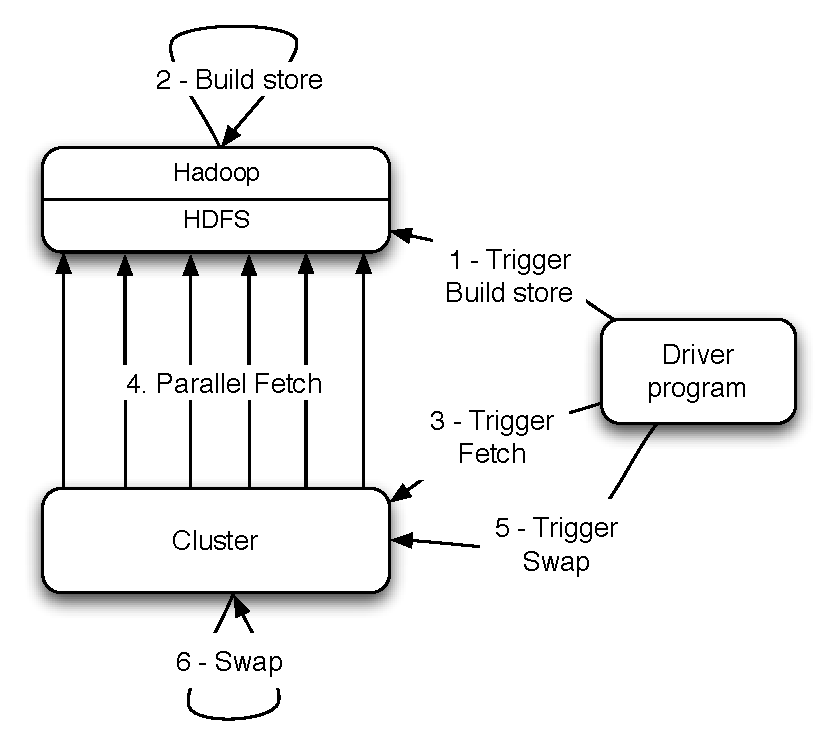
\includegraphics[scale=0.60]{images/cycle.pdf}
  \caption{Read-only data cycle}
  \label{cycle}
\end{figure}

The initiator of this complete fetching and swapping of new data process can be either Azkaban or a standalone driver program. Azkaban\cite{azkaban} is a simple batch scheduler built at \linkedin{} which allows you to schedule Hadoop as well other offline batch jobs. Individual end products schedule batch Hadoop and Pig jobs to run algorithms on the raw data which finally loads the data to \projectname{} as the last step. The last step starts by Azkaban triggering our Hadoop job described in Section \ref{sec:read_only:chunk_generation}. This job generates the data on a per node basis and stores it into HDFS. While streaming the data out onto HDFS we also calculate the checksum on a per node basis. This checksum is calculated by running an MD5 on the individual MD5s of all the chunk files in a node directory. This checksum value is then stored in a special file $.metadata$ in every node folder. 

Once the Hadoop job is complete Azkaban triggers a fetch request on all \projectname{} nodes along with information about the root directory path on HDFS. This request is received by our `administrative service' on every node which then initiates an HDFS client and starts a parallel fetch for the node folder it is responsible for. This data is stored into a new version directory whose version number could either be specified as a parameter by Azkaban or defaulted to (previous version number + 1). While the data is being fetched from HDFS we also calculate the same checksum so as to cross-check it with the stored checksum in the $.metadata$ file. While building this fetch layer we made sure to keep the interface generic so as to support fetching data from non-HDFS locations as well. The other important decision we made here was to adopt the pull model instead of the push model. This allows the \projectname{} node to now throttle the fetches in case of any latency problems. 

The next step after the fetch is complete is to swap the new data-set in and swap the older version out. For Azkaban to know when to initiate a swap it needs to know when the fetch has successfully completed. Since the fetch process can take a long time we provide a hook in the administrative service for Azkaban / standalone program to keep checking so as to get a progress report of how much we have finished fetching. Finally after the fetch is complete Azkaban triggers a swap operation on all nodes. This operation is co-ordinated using a read-write lock in our storage engine. We obtain a write lock when the swap starts during which we do the following - close all open file in the current version directory, change the symbolic link to the new version directory and finally open all chunk files and memory map the indexes. This complete operation doesn't take more than a few milliseconds since it is not dependent on the file size information. To provide global atomic semantics we make sure that all the nodes have successfully swapped their data. If any of the swaps have failed, we run an extra step to rollback the data on the successful nodes.


% ========================== READ-ONLY-STORAGE ENGINE  - COMPLETE DATA CYCLE - SCHEMA CHANGE ==========================================

\subsubsection{Schema upgrades}
\label{sec:read_only:data_cycle:schema_upgrades}

As engineers iterate on their products there are bound to be changes in the underlying data format of the values that they want to expose to the user. Common example of this is if a product wants to add a new dimension to their value. For the same \projectname{} supports the ability to change the schema of the key and value without any downtime. Since read-only data is static and we can do a complete load of the full data-set every time we can easily change the schema during one of our loads. But for the client to transparently handle this change we need to added a special byte in our most used serialization format, Binary JSON, to encode the version of the schema. This same version information is saved in the stores metadata which the clients pick up during bootstrapping. The clients then maintain a mapping from version id to corresponding schema. So if a data fetch takes place with the new schema, during the read we toggle to the right version id and pick up the corresponding schema. Similarly if a rollback of data takes place the client will toggle back to an older version of schema and be able to parse the data with no downtime. 

% ========================== READ-ONLY-STORAGE ENGINE  - COMPLETE DATA CYCLE - REBALANCING ==========================================

\subsubsection{Rebalancing}
\label{sec:read_only:data_cycle:rebalancing}

Rebalancing is a major feature which allows \projectname{} to easily add or rebalance data around on a live cluster without down time. This feature was initially written for the read-write stores but easily fits into the read-only cycle due to the static nature of the data. Our smallest unit of rebalancing is a partition. In other words addition of a new node translates to giving the ownership of some partitions to it. The rebalancing process is run by a rebalancing tool which co-ordinates the full process. The following are the steps that are followed during the addition of a new node. 

\begin{itemize}
	\item Provide the rebalancing tool with the future cluster topology metadata.
	\item Using the future cluster topology metadata, generate list of all primary partitions that need to be moved
	\item Do the following steps for every `batch' of primary partitions. The reason behind moving the partition in small batches is that it makes the process checkpoint-able without having to re-fetch too much data. 
		\begin{itemize}
			\item Generate intermediate cluster topology metadata which is current cluster topology with changes in ownership of `batch' of partitions moved
			\item Use intermediate cluster topology metadata to generate a set of steps that need to be run to finish rebalancing. In this process we also need to take care of all the secondary replica movements that might be required due to the primary partition movement. This plan is a set of donating node id and stealing node id pairs along with the chunk files being moved. 
			\item Initiate asynchronous processes (through the administrative service) on all the stealer nodes which then start stealing chunk files from their corresponding donor nodes. The data is copied into the same version directory which is currently serving live traffic. We also make these nodes to go into a `rebalancing state' thereby not allowing any new fetches and swaps from taking place. 
			
			Here it is important to note that the granularity of the bucket we selected made this process as simple as just a copy of files. If we had defined a bucket to be on a per node basis i.e. have multiple chunks on a per node basis, we would have had to iterate over all the keys on the node and find the correct key set belonging to the moving partition. Further we would then need to merge this key set with the live serving index on the stealer node's end. 
			\item Once the fetches have completed the rebalancing tool updates the intermediate cluster topology on all the nodes while also doing an atomic swap of data on the stealer and donor nodes. 
			
			This topology change information also needs to be propagated to all the upper services using client side routing. We propagate this information as a lazy process where-in the clients still use the old metadata. If they contact a node with a request for a key in a partition which the node is no more responsible the node sends a special exception. This special exception then results in a re-bootstrap step along with a retry of the previous request.
		\end{itemize}
\end{itemize}

The rebalancing tool has also been designed to handle failure scenarios elegantly. Failure during a fetch is not a problem since we haven't swapped the data in. But failure during the swap requires us to rollback the cluster topology to the last good cluster topology while also rolling back the data on the successful nodes. Let us end this section by demonstrating a simple example showing the plan generation. We will run this for the same hash ring shown in Figure \ref{hash} with a store using consistent hashing. We introduce a new node (Node 3) to whom we will initially pass the responsibility of partitions 3. Table \ref{tab:new_node_to_chunk} shows the new chunk mapping, while Table \ref{tab:rebalance_plan} shows the simple plan that would be generated as a part of rebalancing. 

\begin{table}
\begin{center}
    \begin{tabular}{ | c | c | }
    \hline
    Node Id & Chunk files \\ \hline
    0 &  	0\_0, 6\_0, 9\_0,      			5\_1, 8\_1, 11\_1 			\\
   	1 &   	1\_0, 4\_0, 7\_0, 10\_0,      	0\_1, 3\_1, 6\_1,9\_1  		\\
   	2 &    	2\_0, 5\_0, 8\_0, 11\_0,    	1\_1, 4\_1, 7\_1, 10\_1		\\
   	3 &   	3\_0,                         	2\_1 						\\
\hline
    \end{tabular}
\end{center}
 	\caption{New node to chunk mapping}
 	\label{tab:new_node_to_chunk}
\end{table}

\begin{table}
\begin{center}
    \begin{tabular}{ | c | c | c | }
    \hline
    Stealer Node Id & Donor Node Id & Chunks to steal \\ \hline
    3 &  0 & 3\_0, 2\_1	\\
\hline
    \end{tabular}
\end{center}
\caption{Rebalancing plan generated}
\label{tab:rebalance_plan}
\end{table}



% ========================== BENCHMARK ==========================================

\section{Benchmark}
\label{sec:benchmark}

In this section we will present some experiment numbers on a simulated data-set as well as production numbers on two user facing features viz. `People You May Know' (also called PYMK) and `Viewers of this profile also viewed' (also called Browsemaps). We use two metrics to evaluate our system - faster build time and good serving latency. All tests were run on boxes running Linux 2.6.18 with Dual CPU (each having 8 cores running at 2.67 GHz), 24 GB RAM and 6 RAID 10 drives. For the MyISAM tests we ran MySQL Community Edition version 5.0.27. We start by describing the data-sets we used for our benchmarking. 

\begin{itemize}
	\item Random data-set : The key is a long between 0 and a varying number. The value is a fixed 1024 bytes size random string. 
	\item PYMK data-set : On logging into our site, our users are presented with recommendations of other users whom they might know and would connect with. This is presented as a store where they key is the logged in user's member id while the value is a list of integer recommended member ids. Figure \ref{distribution} shows the value size distribution for this store. 
	\item Browsemaps data-set : Browsemaps runs collaborative filtering algorithm on members and shows you similar members when you visit a member's profile. The value is a list of 2 integers, a string and a flot. Similar to PYMK, Figure \ref{distribution} shows the value size distribution for Browsemaps. 
\end{itemize}

\begin{figure}
  \centering
    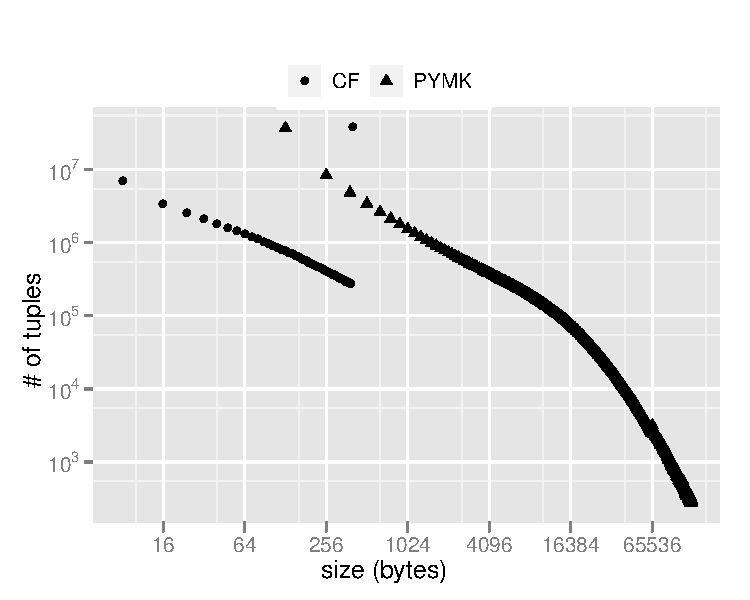
\includegraphics[scale=0.55]{images/data_distribution.pdf}
  \caption{Value size distributions}
  \label{distribution}
\end{figure}

The first metric that we look into is the build times. To do a fair comparison we build all our stores for a single node. The build time in case of our Hadoop job includes the time it takes to generate the chunk mapping (map phase), shuffle the data and finally emit it to the store files (reduce phase). The number of mappers and reducer were kept fixed so as to have same amount of parallelism. This also resulted in fixed number of chunks being generated.

In case of MySQL - MyISAM test the total time only includes the completion of the `LOAD DATA INFILE' command. This does not include the time it took us to extract this data, convert it into TSV format and finally copy it over to the node running MySQL single instance. Some other optimizations we did to make MySQL faster include - (a) Increasing the MySQL bulk insert buffer size and MyISAM specific sort buffer size to 256 MB each (b) Delaying the re-creation of the index to a latter time by running `ALTER TABLE...DISABLE KEYS' statement before the load. 

Besides the B$^{+}$ tree structure built inside MySQL, we wanted to try to build our own B$^{+}$ tree structure tailored to Hadoop. Instead of generating chunk files in every reducer step, we generate a B$^{+}$ tree. This tree contains of a single data file (similar to the chunk data file) and a set of index files corresponding to every level of the tree. The bulk loading of the tree is done in blocks (of size $b$) i.e. we first finish the lower level's block and only then initialize a block at the next level. We then apply this rule recursively for every level as the sorted elements stream through. This bulk loading approach is efficient in that it does not require us to buffer any values in memory and can directly write to the level based index files. 

The graph in Figure \ref{build} is the build time in seconds for the above three scenarios as we increased the size of the input data-set. The block size $b$ for the B$^{+}$ was set to 340. We chose this value since our keys were 12 bytes (8 byte MD5 and 4 byte offset) long and the page size was 4096 bytes. This meant the best block size would be approximately 4096/12 $\sim$ 340. As is clearly evident MySQL takes a really long time even after being alloted a huge buffer size. The optimized B$^{+}$ on the other hand performs very well initially for small sizes but starts to deviate for larger sizes due to the extra I/O that it needs to do. In particular it needs to do extra disk writes equal to the data in the higher levels of the tree. For a fixed block size, the extra disk writes is linear with the number of tuples. The big disadvantage of the B$^{+}$ tree approach is that the serving latency is very sensitive to the block size $b$. Unfortunately setting the right value of $b$ is machine specific and hence error prone. 

\begin{figure}
  \centering
    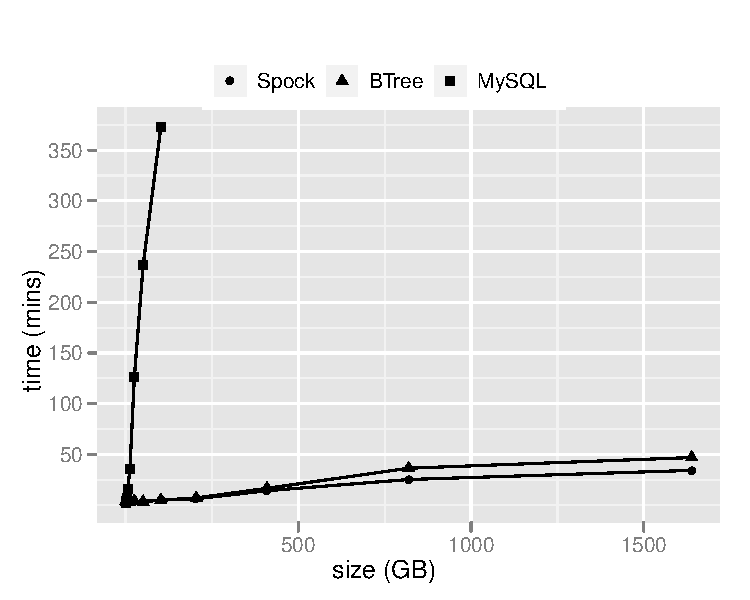
\includegraphics[scale=0.55]{images/build.pdf}
  \caption{Build time vs size of data}
  \label{build}
\end{figure}

The next metric we benchmark is the search latency. For the random data-set we used 10 million requests with simulated values following an uniform distribution. For the PYMK and Browsemaps data-set we took a snapshot of member activity from our live Kafka stream on one of the high traffic days and used that data to generate performance numbers.

We first try to understand the performance implications of binary search vs interpolation search. In particular we were interested in measuring how fast the index can get paged into the operating system's page cache and whether the search algorithm can help with that. We ran tests on a 100GB of data on a single node with the page cache being flushed between test runs. The graph in Figure \ref{search} plots the median latency vs time. As is evident from the graph even though binary search initially starts with a very high median latency the slope of the line is steeper compared to that of interpolation search. This is because we found binary search algorithm did an average of 17.5 lookups thereby touching way more parts of the index from the very beginning. Compared to that interpolation search does only 4 lookups which hence results in an initial low search latency but comes at the expense that most parts of all the indexes are un-cached for a longer time. Our production systems are currently running on binary search due to faster cache warming process.  

\begin{figure}
  \centering
    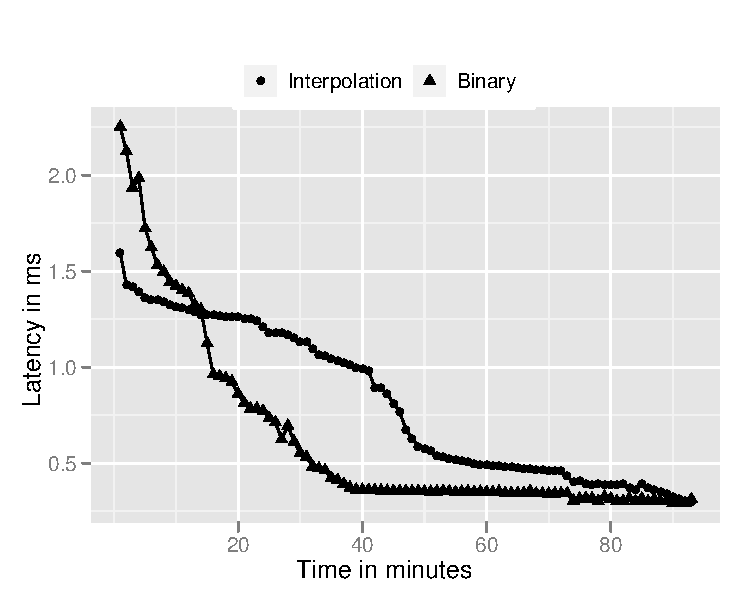
\includegraphics[scale=0.55]{images/search_1node.pdf}
  \caption{Search Latency vs Time}
  \label{search}
\end{figure}

We ran the same 100 GB data-set through MySQL to get its performance numbers. Following table summaries the performance difference for a fixed throughput of 1000 queries per second. 

\begin{center}
    \begin{tabular}{ | c | c | c |  }
    \hline
     & MySQL & \projectname{} \\ \hline
    Median &   0.12 ms &  0.028	ms \\
	99th Percentile	& 45 ms & 36 ms \\
\hline
    \end{tabular}
\end{center}

To test whether the system scales well with the number of boxes, we present the latency numbers for the same random data-set but spread over 16 boxes. The data was fetched by \projectname{} at a steady rate bound by the disk or network. In our scenario we saturated the 1 Gbit line between HDFS and \projectname{} nodes. We ran the tests for both uniform as well as zipfian distribution (generation of which is further described in \cite{gray}). In particular we make sure that the `hot' elements are queried together since that simulates the general site visiting patterns of some users frequently coming to our site and generating a lot of activity. Figure \ref{16search} shows the max of the median latency of individual nodes versus different data-sizes. The `hotness' of some keys makes it very cacheable thereby giving an overall lower latency compared to the uniform distribution. 

\begin{figure}
  \centering
    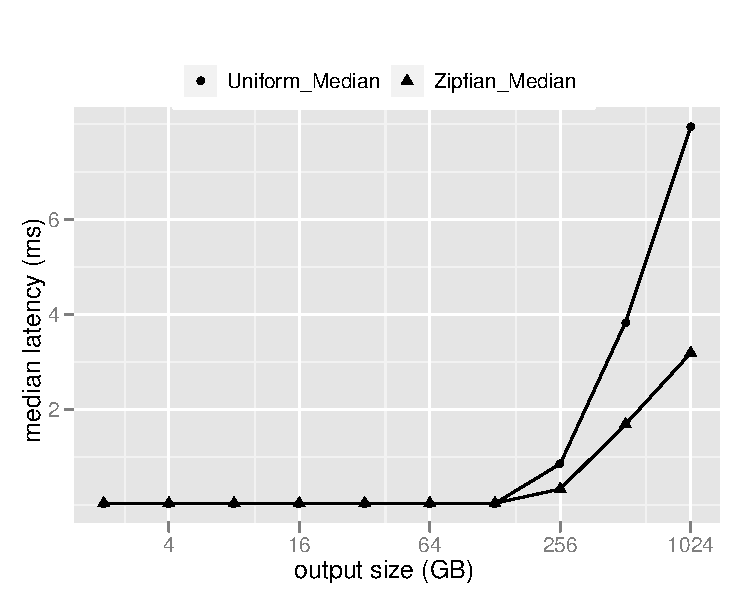
\includegraphics[scale=0.55]{images/search_16node.pdf}
  \caption{Search Latency vs Data size for 16 nodes}
  \label{16search}
\end{figure}


We finally present the latency numbers for PYMK and Browsemaps on our production cluster in Figure \ref{production}. This shows the average latency on the server side across all nodes immediately after a new data swap. Browsemaps has a high latency primarily because of the data size being larger than that of PYMK.

\begin{figure*}
  \centering
%    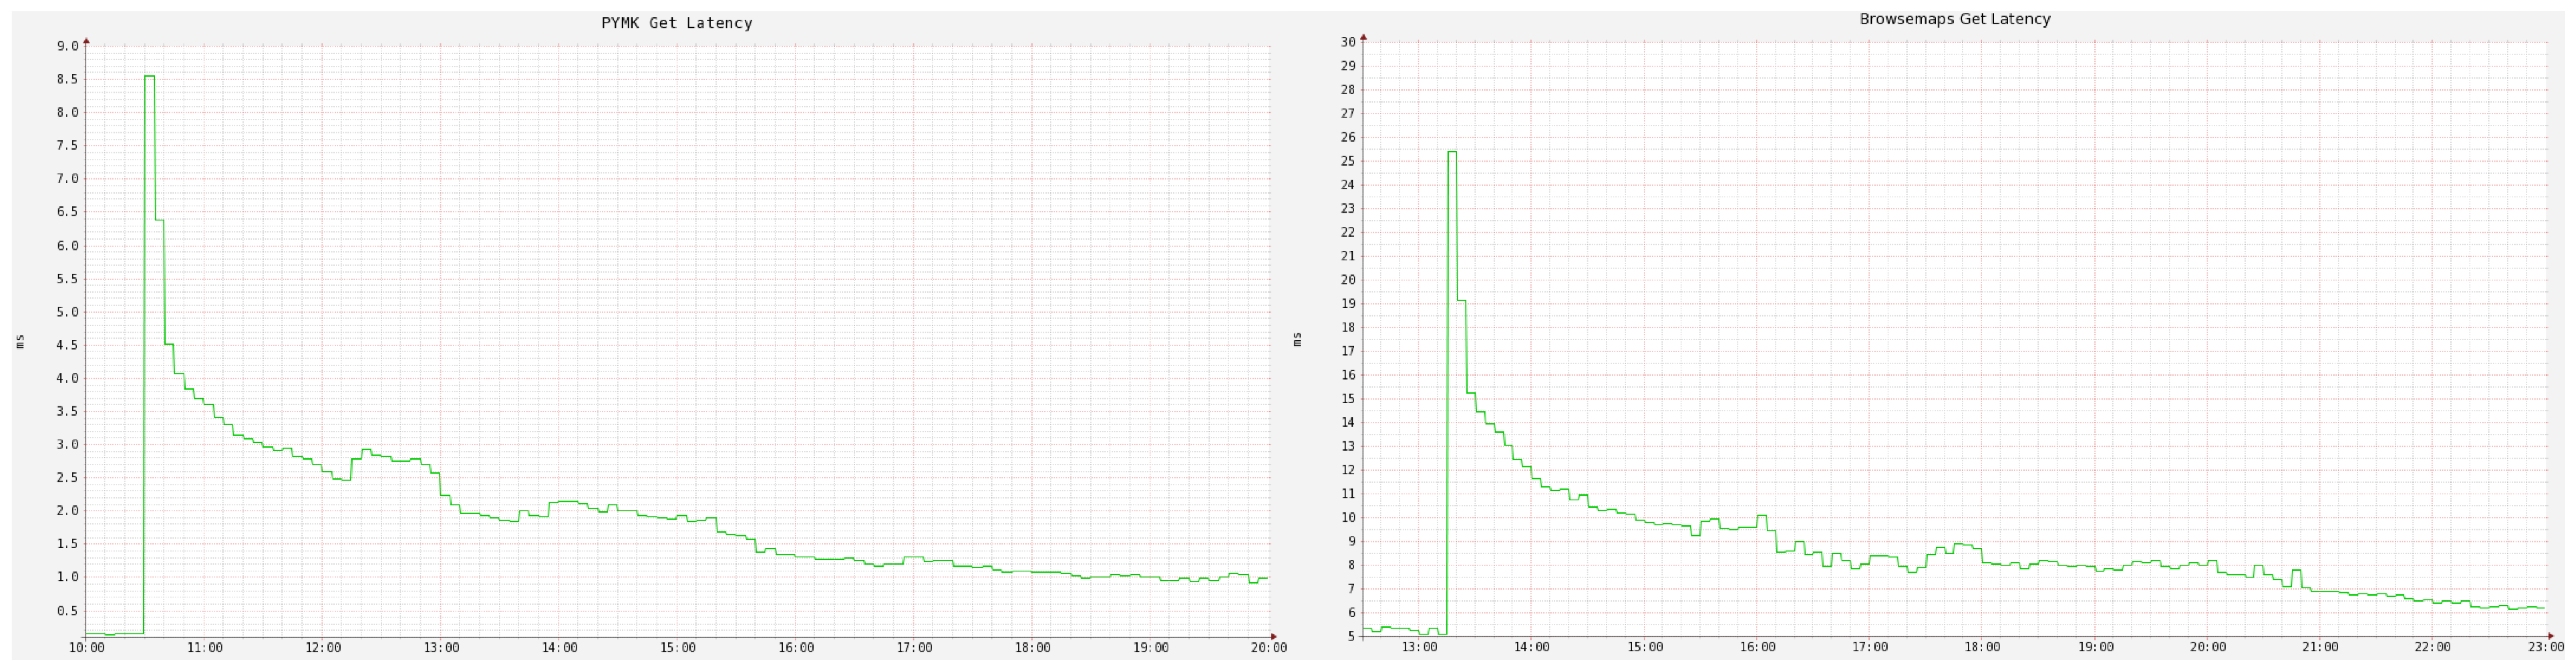
\includegraphics[scale=0.23]{images/get_latency.pdf}
  \caption{Latency vs Time for PYMK and Browsemaps}
  \label{production}
\end{figure*}




% ========================== CONCLUSION  ==========================================

\section{Conclusion / Future Work}
\label{sec:conclusion}

In this paper we present a low-latency bulk loading system capable of serving multiple TBs of data. By moving the index construction offline to a batch system like Hadoop, we make our serving layer's performance more reliable. \\linkedin{}{} has successfully been running read-only \projectname{} clusters for the past 2 years. It has become an integral part of the product eco-system with various engineers also using it frequently for quick prototypes of products. 

There are still some interesting functionalities that we would like to add to the read-only storage pipeline. Firstly, we want to add support for incremental loads. We do have an initial prototype for in which we create patches for the data files on the Hadoop side (by comparing against the snapshot of the previously loaded data still in HDFS) and then apply these on the \projectname{} side during the fetch. We don't do any patch generation for the index files and just send them over since these are relatively small. We are still exploring the use of this functionality since most of our current users are recommendation products where the values, represented by floats for probabilities, generally change between iterations for most users. 

Another important feature that we want to add to the fetch pipeline is the ability to only get one replica of the data from HDFS and then propagate it further on the \projectname{} node. The motivation for this is that most \projectname{} setups might run in a data-center separate from the one running Hadoop (and HDFS). In such a scenario optimizing the amount of data being transferred between data-centers can be a great plus. We have also tried compressing the complete data before storing it in HDFS and then un-compressing this on the fly on the \projectname{} side. Unfortunately this isn't that helpful in scenarios where the users have decided to use the per-key based compression since we are already dealing with compressed data. But copying just one replica of the data would definitely save inter-data-center bandwidth. 

Finally we would definitely like to explore some more index structures which would make lookups faster and can be built in Hadoop easily. In particular a lot of work has been done in the area of cache oblivious trees, like van Emde Boas trees, which requires no knowledge of page size to get optimal cache performance. 

\bibliographystyle{plain}
\bibliography{voldemort}

\end{document}

